\documentclass{beamer}
\mode<presentation> { \setbeamercovered{} }

\usetheme{Warsaw}
\usecolortheme{seahorse}
\setbeamertemplate{navigation symbols}{}
\setbeamertemplate{caption}{\raggedright\scriptsize\insertcaption\par}
\setbeamertemplate{headline}{%
\leavevmode%
    \begin{beamercolorbox}[wd=\paperwidth,ht=3ex,dp=1.9ex]{palette quaternary}%
    \insertsectionnavigationhorizontal{\paperwidth}{\hskip0pt plus1fill}{\hskip0pt plus1fill}
    \end{beamercolorbox}%
}
\setbeamercolor{background canvas}{bg=}
% \setbeamerfont{footnote}{size=\tiny}
\usepackage{beamerthemesplit}
\usepackage{lmodern}
\usepackage{bold-extra}
\usepackage{pgf}
\usepackage{epsfig}
\usepackage{epstopdf}
\usepackage{graphicx}
\usepackage{slashbox}
\usepackage{url}
\usepackage{listings}
\usepackage{polski}
\usepackage[utf8]{inputenc}
\usepackage[absolute,overlay]{textpos}
\usepackage{graphicx}
\usepackage[style=verbose,backend=biber,sorting=none]{biblatex}
\usepackage[version=3]{mhchem}
\usepackage{xspace}
\usepackage{multirow}
\usepackage{bm}
\addbibresource{mmc.bib}

\newcommand{\IR}{\bbold R}
\newcommand{\HH}{\ce{H2}\xspace}
\def\Rset{\mathbb{R}}
\def\Zset{\mathbb{Z}}
\newcommand{\refbr}[1]{(\ref{#1})}
\newcommand{\beq}{\begin{equation}}
\newcommand{\eeq}{\end{equation}}
\newcommand{\und}[1]{\underline{#1}}
\newcommand\pro{\item[$+$]}
\newcommand\con{\item[$-$]}
\newcounter{saveenumi}
\newcommand{\seti}{\setcounter{saveenumi}{\value{enumi}}}
\newcommand{\conti}{\setcounter{enumi}{\value{saveenumi}}}
\lstset{
    numbers=left,
    breaklines=true,
    tabsize=2,
  numberstyle=\color{gray}\footnotesize,
    basicstyle=\small\ttfamily,
}
\newcommand{\ttbf}[1]{{\tt \textbf{#1}}}

% \AtBeginSection{
%   \begin{frame}
%   \vfill
%   \centering
%   \begin{beamercolorbox}[sep=8pt,center,shadow=true,rounded=true]{title}
%     \usebeamerfont{title}\insertsectionhead\par%
%   \end{beamercolorbox}
%   \vfill
%   \end{frame}
% }

\hypersetup{
   pdftitle={Prospects of green hydrogen in Poland: A techno-
economic analysis using a Monte Carlo approach},
   pdfauthor={Jakub Ostrzołek},
   pdfborder={0 0 0}
}

\title[Prospects of green hydrogen in Poland \insertframenumber/\inserttotalframenumber]{
  Recenzja: \\%
  \emph{Prospects of green hydrogen in Poland:
  A techno-economic analysis using a Monte Carlo approach}}
\author[Jakub Ostrzołek]{\textbf{Jakub Ostrzołek} \\%
\footnotesize Autorzy pracy źródłowej: Pablo Benalcazar, Aleksandra Komorowska}
\institute{Instytut Automatyki i Informatyki Stosowanej\\%
Politechnika Warszawska}

\begin{document}

\frame{\titlepage}

\frame{\tableofcontents\frametitle{Plan prezentacji}}

\section{Wprowadzenie do tematu}

\begin{frame}
	\frametitle{Motywacja}
	Nadchodzące zmiany energetyczne:
	\begin{enumerate}
		\item EU: plan osiągnięcia nautralności klimatycznej do 2050
		      \begin{itemize}
			      \item $17.5 \, GW$ łącznej mocy elektrolizerów \HH do 2025
			      \item produkcja + import 10 mln ton \HH do 2030
			      \item brak emisji gazów cieplarnianych do 2050
		      \end{itemize}
		\item \emph{Polityka Energetyczna Polski do 2040}
		\item \emph{Polska Strategia Wodorowa do roku 2030}
	\end{enumerate}
	Niewiele analiz rozwojowych gospodarki \HH na terenie Polski w stosunku do państw zachodnich. Brak analiz MC.
\end{frame}

\begin{frame}
	\frametitle{Zastosowania \HH}
	Po co nam \HH?
	\begin{itemize}
		\item posiada dużą tzw. \emph{gęstość energii}

		      \begin{tabular}{ l r }
			      tradycyjne baterie & $0.1 - 0.27 \; kWh/kg$ \\
			      benzyna            & $13 \; kWh/kg$         \\
			      \HH ($700 \; bar$) & $39.6 \; kWh/kg$
		      \end{tabular}
		\item można go tworzyć w pikach produkcji energii a potem zużyć o dogodnej porze
		\item można efektywnie transportować energię na duże odległości
		\item inne zastosowania, np: przemysł, transport, ogrzewanie
	\end{itemize}
\end{frame}

\begin{frame}
	\frametitle{Produkcja \HH}
	Rodzaje produkcji \HH
	\begin{enumerate}
		\item \emph{szary} -- z gazu naturalnego lub metanu ($\sim 97\%$)
		\item \emph{niebieski} -- szary + przechwytywanie \ce{CO2}
		\item \emph{fioletowy} -- z energii atomowej
		\item \textbf{\emph{zielony}} -- z energii odnawialnej
	\end{enumerate}
\end{frame}


\begin{frame}
	\frametitle{Efektywność}
	Czynniki wpływające na efektywność farmy \HH
	\begin{itemize}
		\item farma = elektrownia odnawialna + elektrolizer \HH
		\item sprzęt: elektrolizery (PEM), elektrownie (wiatrowe, PV, ...)
		\item warunki pogodowe, geologiczne
		\item koszta: CAPEX + OPEX (obsługa, prąd, woda, utrzymanie)
		\item metryka?
	\end{itemize}
\end{frame}

\section{Model}

\begin{frame}
	\setbeamercovered{transparent}
	\frametitle{LCOH}
	Levelized Cost of Hydrogen (LCOH)
	\begin{align}
		LCOH     & = \frac{(C_{CC} \times CRF)
		+ C_{O\&M} + C_{REP}}{M_{\HH}} \nonumber                         \\
		\pause
		CRF      & =  \frac{i \times (1 + i)^N}{(1 + i)^N - 1} \nonumber \\
		\pause
		C_{CC}   & =  P_{el} \times I_{el} \nonumber                     \\
		\pause
		C_{O\&M} & =  (\tau \times P_{el} \times u_{el} \times c_e)
		+ (\gamma \times M_{\HH} \times c_w)
		+ (C_{CC} \times \phi) \nonumber                                 \\
		\pause
		M_{\HH}  & =  \frac{\tau \times P_{el}
		\times u_{el}}{E_{el}} \nonumber                                 \\
		\pause
		C_{REP}  & =  \frac{i \times (1 + i)^N}{(1 + i)^N - 1}
		\times \frac{C_{TotalRep}}{(1+i)^t} \nonumber
	\end{align}
\end{frame}

\begin{frame}
	\frametitle{Capital Recovery Factor?}
	\begin{align}
		LCOH     & = \frac{(C_{CC} \boldsymbol{\times CRF})
		+ C_{O\&M} + C_{REP}}{M_{\HH}} \nonumber                                      \\
		CRF      & =  \frac{\boldsymbol{i} \times (1 + i)^N}{(1 + i)^N - 1} \nonumber \\
		C_{CC}   & =  P_{el} \times I_{el} \nonumber                                  \\
		C_{O\&M} & =  (\tau \times P_{el} \times u_{el} \times c_e)
		+ (\gamma \times M_{\HH} \times c_w)
		+ (C_{CC} \times \phi) \nonumber                                              \\
		M_{\HH}  & =  \frac{\tau \times P_{el}
		\times u_{el}}{E_{el}} \nonumber                                              \\
		C_{REP}  & =  \frac{i \times (1 + i)^N}{(1 + i)^N - 1}
		\times \frac{C_{TotalRep}}{(1+i)^t} \nonumber
	\end{align}
\end{frame}

\begin{frame}
	\frametitle{Capital Recovery Factor?}

	\begin{table}
		\begin{tabular}{|| c | c || c c c c ||}
			\hline
			\multicolumn{2}{||c||}{} & \multicolumn{4}{c||}{$N$}                                 \\
			\cline{3-6}
			\multicolumn{2}{||c||}{} & 10                        & 20    & 30    & 40            \\ [0.5ex]
			\hline\hline
			\multirow{9}{*}{$i$}     & 0.1                       & 0.163 & 0.117 & 0.106 & 0.102 \\
			\cline{2-6}
			                         & 0.2                       & 0.239 & 0.205 & 0.201 & 0.200 \\
			\cline{2-6}
			                         & 0.3                       & 0.323 & 0.302 & 0.300 & 0.300 \\
			\cline{2-6}
			                         & 0.4                       & 0.414 & 0.400 & 0.400 & 0.400 \\
			\cline{2-6}
			                         & 0.5                       & 0.509 & 0.500 & 0.500 & 0.500 \\
			\cline{2-6}
			                         & 0.6                       & 0.606 & 0.600 & 0.600 & 0.600 \\
			\cline{2-6}
			                         & 0.7                       & 0.703 & 0.700 & 0.700 & 0.700 \\
			\cline{2-6}
			                         & 0.8                       & 0.802 & 0.800 & 0.800 & 0.800 \\
			\cline{2-6}
			                         & 0.9                       & 0.901 & 0.900 & 0.900 & 0.900 \\ [1ex]
			\hline
		\end{tabular}
		\centering
		\caption{$CRM$ w zależności od $i$ oraz $N$}
	\end{table}
\end{frame}

\begin{frame}
	\frametitle{Utilization rate?}
	\begin{align}
		LCOH     & = \frac{(C_{CC} \times CRF)
		+ C_{O\&M} + C_{REP}}{M_{\HH}} \nonumber                                 \\
		CRF      & =  \frac{i \times (1 + i)^N}{(1 + i)^N - 1} \nonumber         \\
		C_{CC}   & =  P_{el} \times I_{el} \nonumber                             \\
		C_{O\&M} & =  (\tau \times P_{el} \times \boldsymbol{u_{el}} \times c_e)
		+ (\gamma \times M_{\HH} \times c_w)
		+ (C_{CC} \times \phi) \nonumber                                         \\
		M_{\HH}  & =  \frac{\tau \times P_{el}
		\times u_{el}}{E_{el}} \nonumber                                         \\
		C_{REP}  & =  \frac{i \times (1 + i)^N}{(1 + i)^N - 1}
		\times \frac{C_{TotalRep}}{(1+i)^t} \nonumber
	\end{align}
\end{frame}

\begin{frame}
	\frametitle{Replacement costs?}
	\begin{align}
		LCOH     & = \frac{(C_{CC} \times CRF)
		+ C_{O\&M} + C_{REP}}{M_{\HH}} \nonumber                                         \\
		CRF      & =  \frac{i \times (1 + i)^N}{(1 + i)^N - 1} \nonumber                 \\
		C_{CC}   & =  P_{el} \times I_{el} \nonumber                                     \\
		C_{O\&M} & =  (\tau \times P_{el} \times u_{el} \times c_e)
		+ (\gamma \times M_{\HH} \times c_w)
		+ (C_{CC} \times \phi) \nonumber                                                 \\
		M_{\HH}  & =  \frac{\tau \times P_{el}
		\times u_{el}}{E_{el}} \nonumber                                                 \\
		C_{REP}  & = \boldsymbol{\sum\limits_t} \frac{i \times (1 + i)^N}{(1 + i)^N - 1}
		\times \frac{C_{TotalRep}}{(1+i)^t} \nonumber
	\end{align}
\end{frame}

\begin{frame}
	\frametitle{Model}
	\begin{figure}
		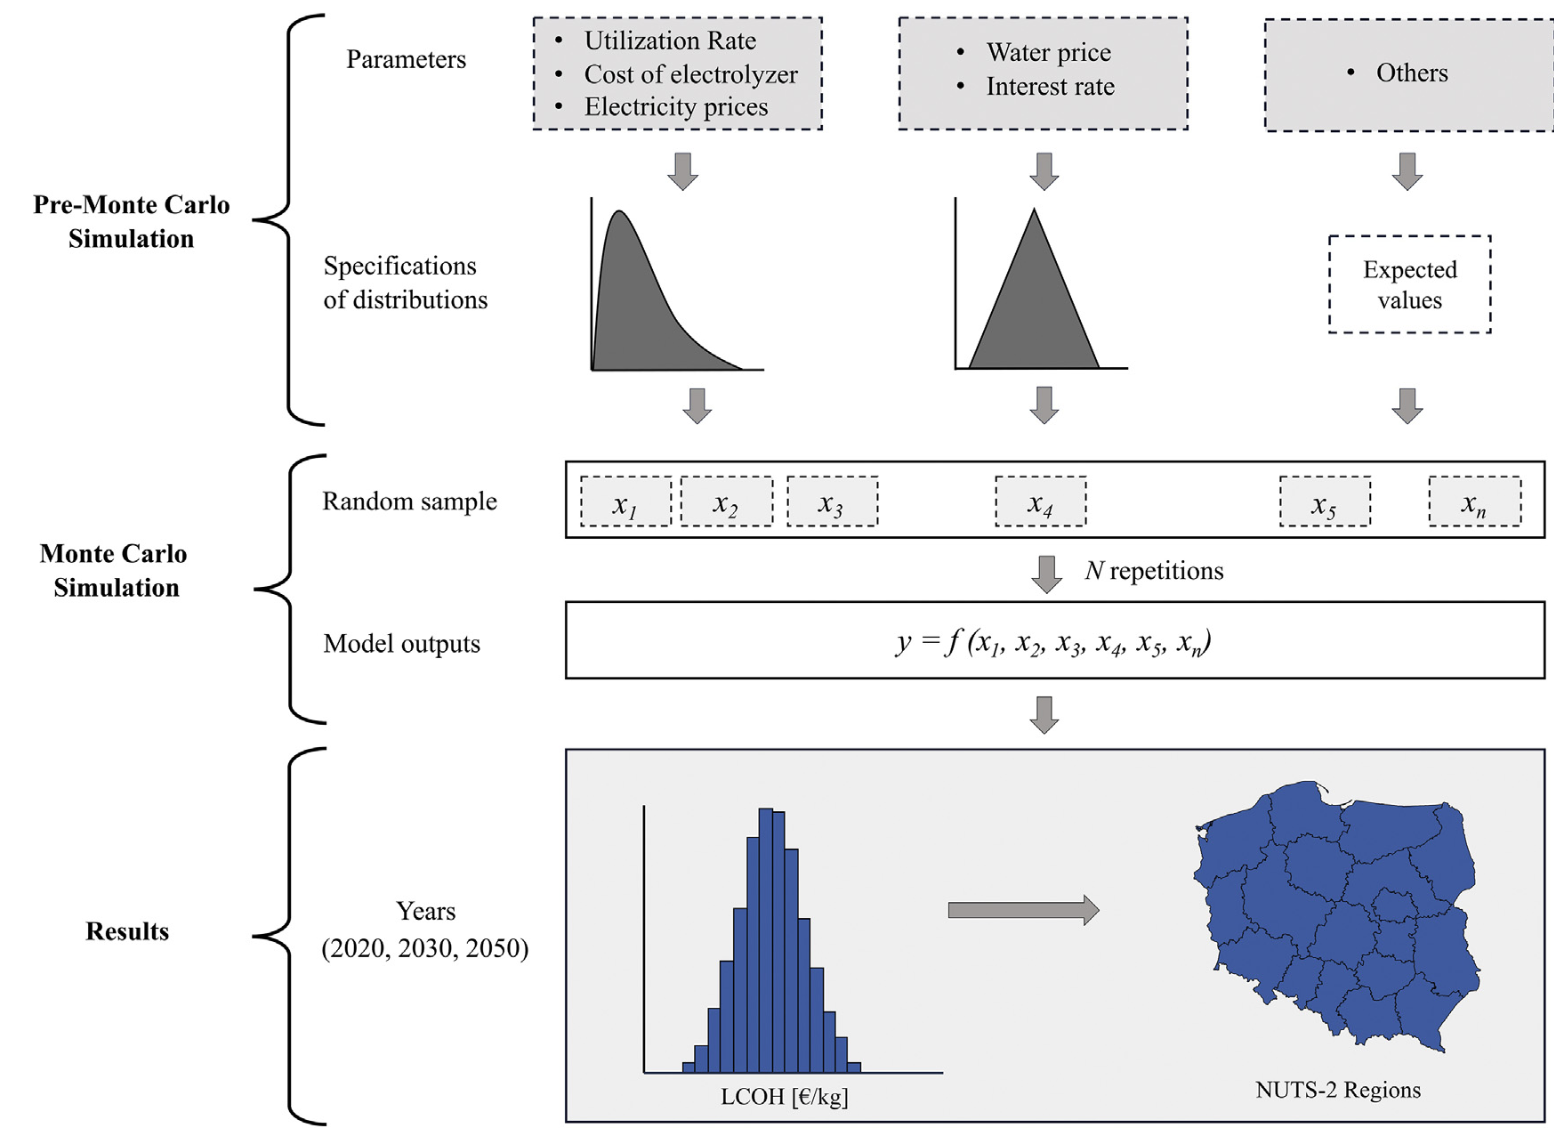
\includegraphics[width=0.82\textwidth]{mmc-diag.png}
		\caption{Diagram modelu}
		\centering
	\end{figure}
\end{frame}


\begin{frame}
	\frametitle{Stałe}
	\begin{figure}
		\begin{center}
			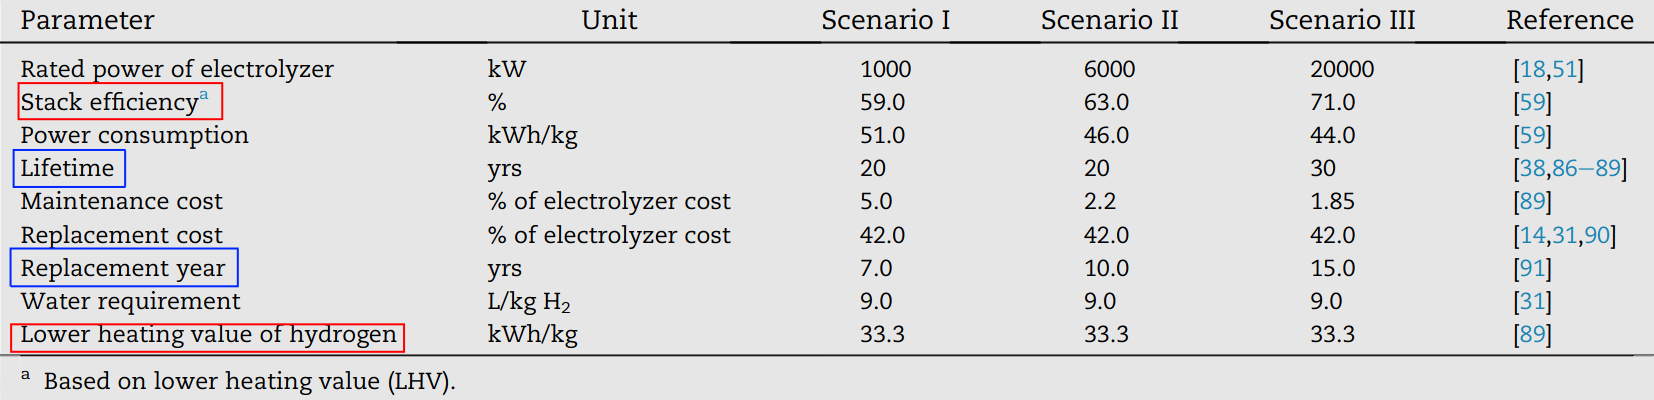
\includegraphics[width=\textwidth]{mmc-constants-annotated.png}
		\end{center}
		\caption{Wartości stałych}
	\end{figure}
\end{frame}

\begin{frame}
	\frametitle{Stałe}
	\begin{align}
		LCOH     & = \boldsymbol{\frac{(C_{CC} \times CRF)
		+ C_{O\&M} + C_{REP}}{M_{\HH}}} \nonumber                                                      \\
		CRF      & =  \frac{i \times (1 + i)^{\boldsymbol{N}}}{(1 + i)^{\boldsymbol{N}} - 1} \nonumber \\
		C_{CC}   & =  \boldsymbol{P_{el}} \times I_{el} \nonumber                                      \\
		C_{O\&M} & =  (\boldsymbol{\tau} \times \boldsymbol{P_{el}} \times u_{el} \times c_e)
		+ (\boldsymbol{\gamma} \times \boldsymbol{M_{\HH}} \times c_w)
		+ (\boldsymbol{C_{CC}} \times \boldsymbol{\phi}) \nonumber                                     \\
		M_{\HH}  & =  \frac{\boldsymbol{\tau} \times \boldsymbol{P_{el}}
		\times u_{el}}{\boldsymbol{E_{el}}} \nonumber                                                  \\
		C_{REP}  & =  \frac{i \times (1 + i)^{\boldsymbol{N}}}{(1 + i)^{\boldsymbol{N}} - 1}
		\times \frac{\boldsymbol{C_{TotalRep}}}{(1+i)^t} \nonumber
	\end{align}
\end{frame}

\begin{frame}
	\frametitle{Zmienne}
	\begin{figure}
		\begin{center}
			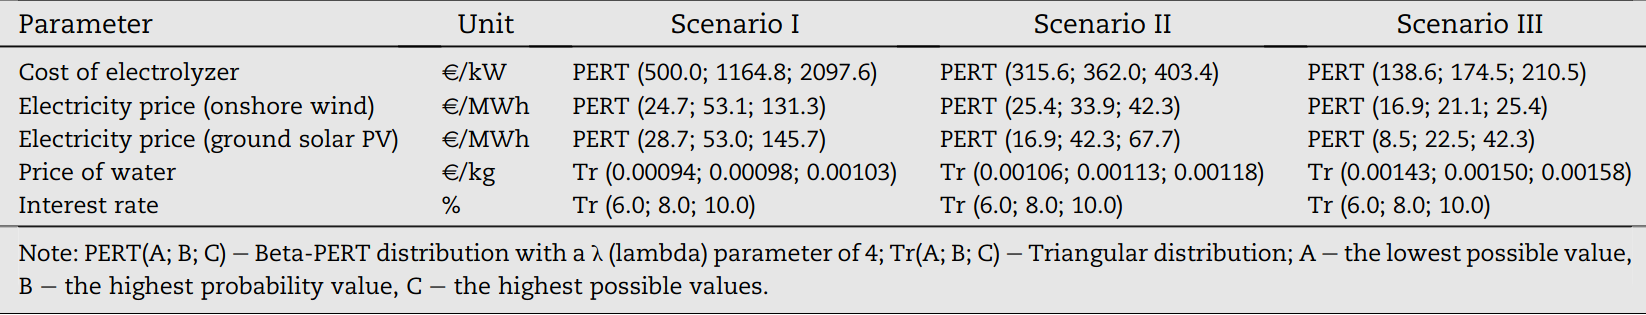
\includegraphics[width=\textwidth]{mmc-variables.png}
		\end{center}
		\caption{Wartości zmiennych}
	\end{figure}
	\pause
	Utilization rate $u_{el}$???
\end{frame}

\begin{frame}
	\frametitle{Gdzie jest $u_{el}$?}
	\begin{figure}
		\begin{center}
			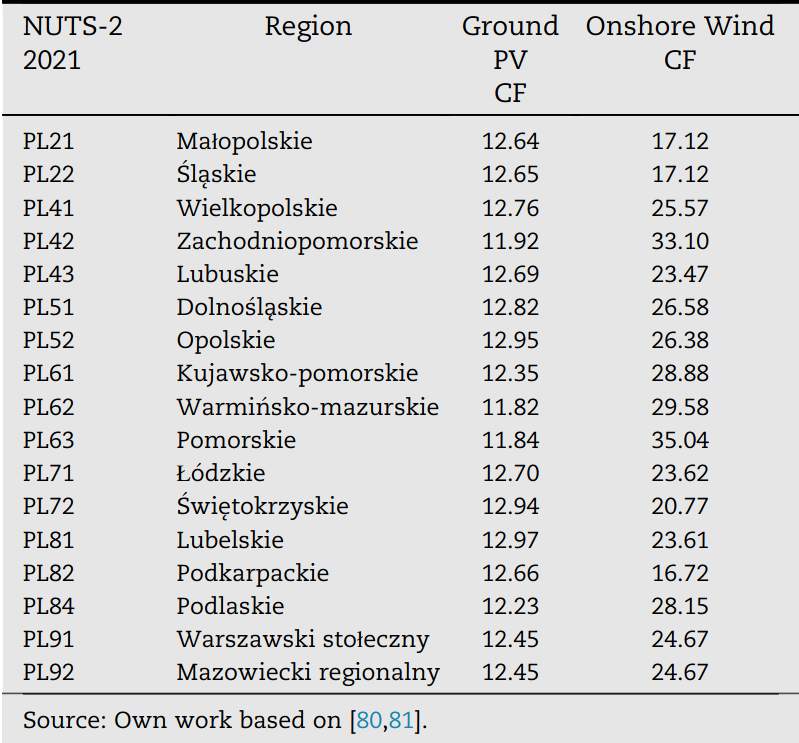
\includegraphics[width=0.6\textwidth]{mmc-cf-table.png}
		\end{center}
		\caption{Średnie współczynniki wydajności ,,capacity factor'' (CF)}
	\end{figure}
\end{frame}

\begin{frame}
	\frametitle{Gdzie jest $u_{el}$?}
	\begin{columns}
		\begin{column}{0.5\textwidth}
			\begin{figure}
				\begin{center}
					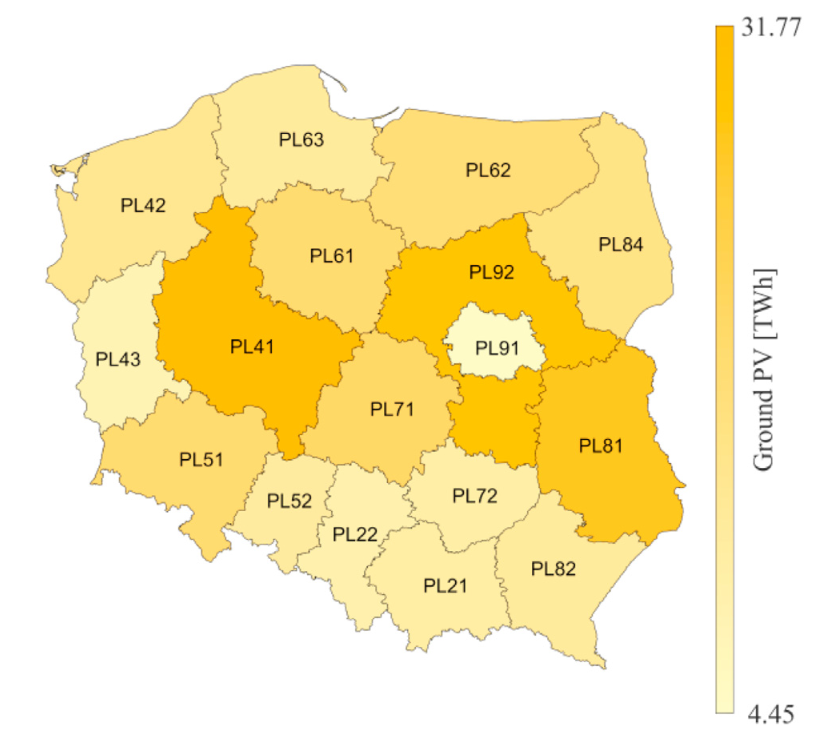
\includegraphics[width=\textwidth]{mmc-cf-pv.png}
				\end{center}
				\caption{Mapy średnich CF dla PV}
			\end{figure}
		\end{column}
		\begin{column}{0.5\textwidth}
			\begin{figure}
				\begin{center}
					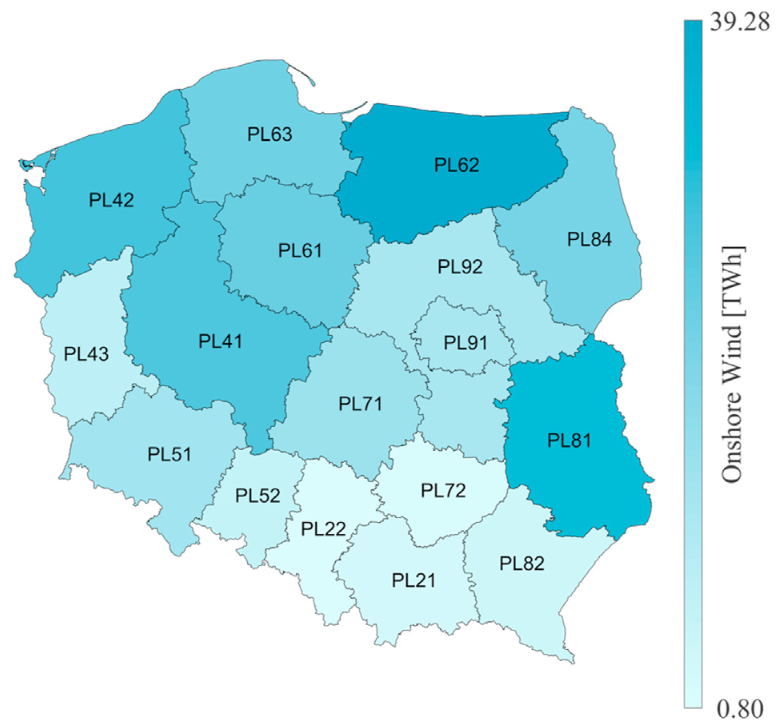
\includegraphics[width=\textwidth]{mmc-cf-wind.png}
				\end{center}
				\caption{Mapy średnich CF dla elektrowni wiatrowych}
			\end{figure}
		\end{column}
	\end{columns}
\end{frame}

\begin{frame}
	\frametitle{Gdzie jest $u_{el}$?}
	\pause
	\textbf{Nigdzie.}
\end{frame}

\section{Wyniki}

\begin{frame}
	\frametitle{Mapy LCOH}
	\begin{figure}
		\begin{center}
			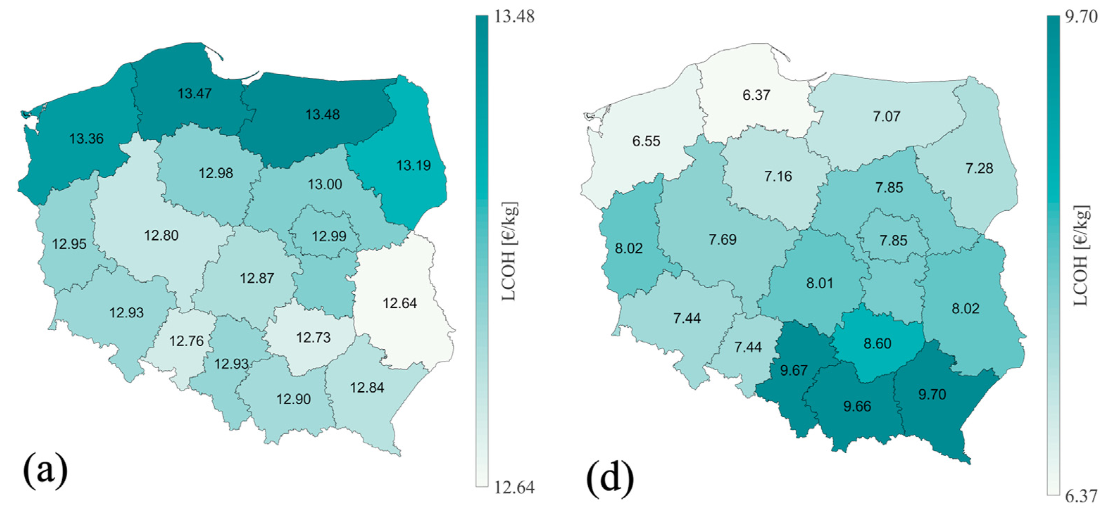
\includegraphics[width=\textwidth]{mmc-results-maps-1.png}
		\end{center}
		\caption{Mapa mediany LCOH -- scenariusz 1 (lewo - PV, prawo - wiatr)}
	\end{figure}
\end{frame}

\begin{frame}[noframenumbering]
	\frametitle{Mapy LCOH}
	\begin{figure}
		\begin{center}
			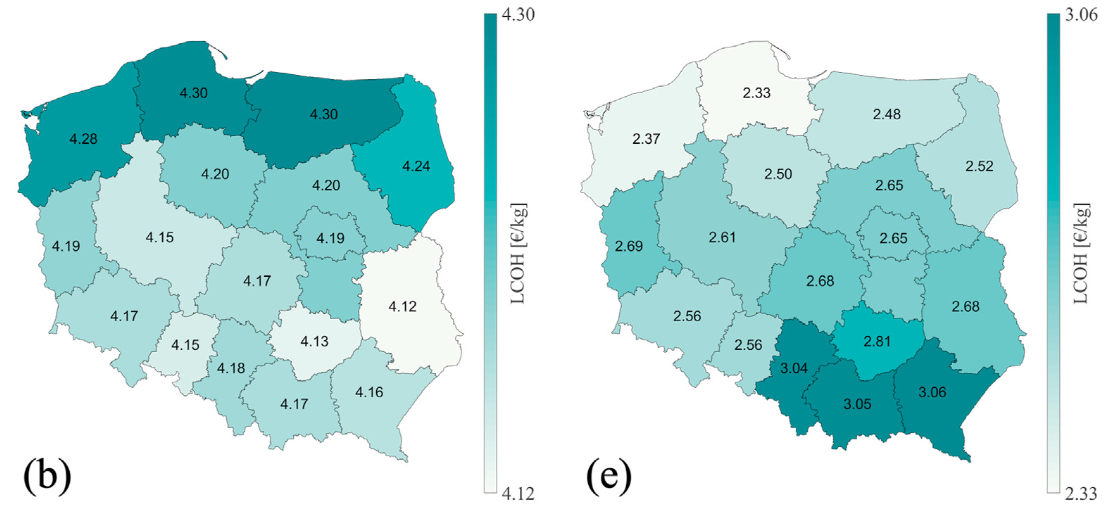
\includegraphics[width=\textwidth]{mmc-results-maps-2.png}
		\end{center}
		\caption{Mapa mediany LCOH -- scenariusz 2 (lewo - PV, prawo - wiatr)}
	\end{figure}
\end{frame}

\begin{frame}[noframenumbering]
	\frametitle{Mapy LCOH}
	\begin{figure}
		\begin{center}
			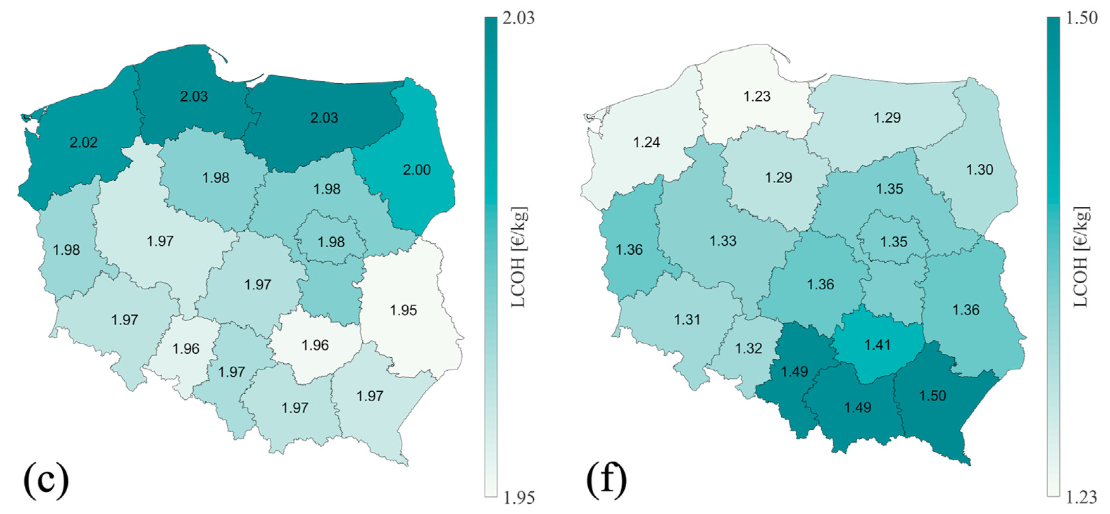
\includegraphics[width=\textwidth]{mmc-results-maps-3.png}
		\end{center}
		\caption{Mapa mediany LCOH -- scenariusz 3 (lewo - PV, prawo - wiatr)}
	\end{figure}
\end{frame}

\begin{frame}
	\frametitle{Rozkłady LCOH}
	\begin{figure}
		\begin{center}
			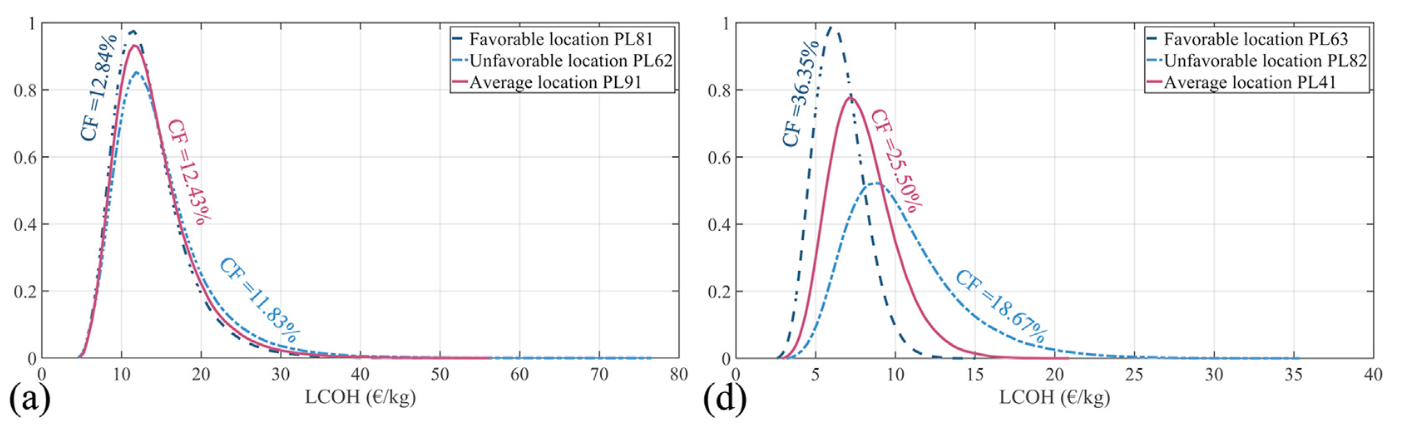
\includegraphics[width=\textwidth]{mmc-results-charts-1.png}
		\end{center}
		\caption{Rozkład LCOH -- scenariusz 1 (lewo - PV, prawo - wiatr)}
	\end{figure}
\end{frame}

\begin{frame}[noframenumbering]
	\frametitle{Rozkłady LCOH}
	\begin{figure}
		\begin{center}
			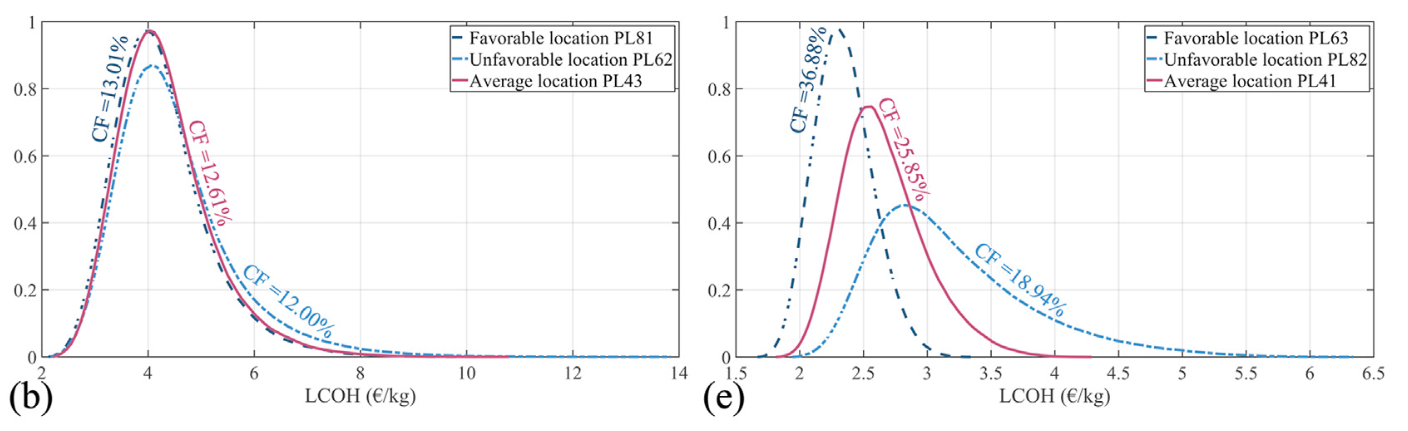
\includegraphics[width=\textwidth]{mmc-results-charts-2.png}
		\end{center}
		\caption{Rozkład LCOH -- scenariusz 2 (lewo - PV, prawo - wiatr)}
	\end{figure}
\end{frame}

\begin{frame}[noframenumbering]
	\frametitle{Rozkłady LCOH}
	\begin{figure}
		\begin{center}
			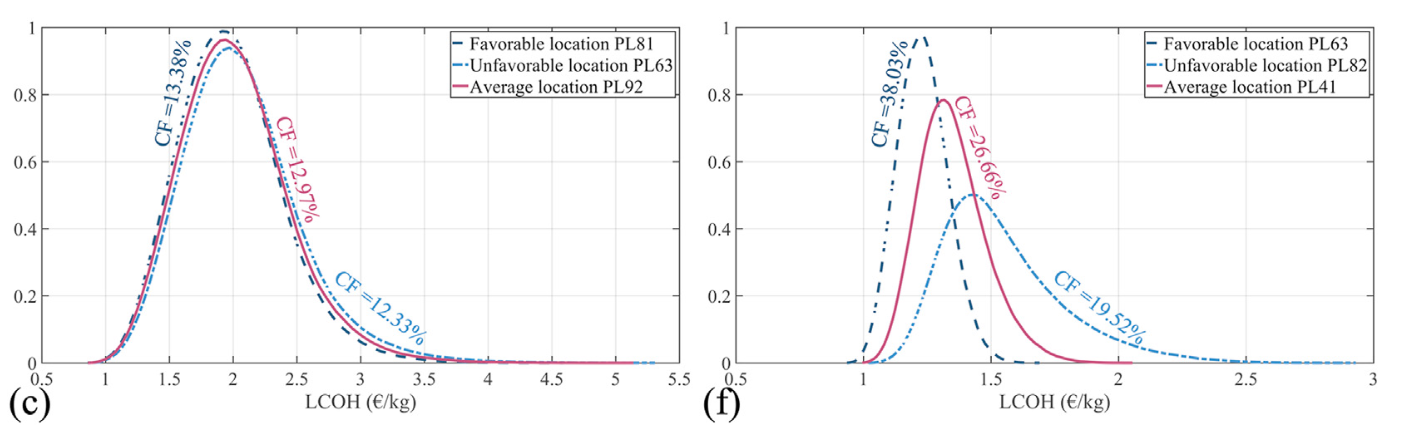
\includegraphics[width=\textwidth]{mmc-results-charts-3.png}
		\end{center}
		\caption{Rozkład LCOH -- scenariusz 3 (lewo - PV, prawo - wiatr)}
	\end{figure}
\end{frame}


\begin{frame}
	\frametitle{Analiza wrażliwości}
	\begin{figure}
		\begin{center}
			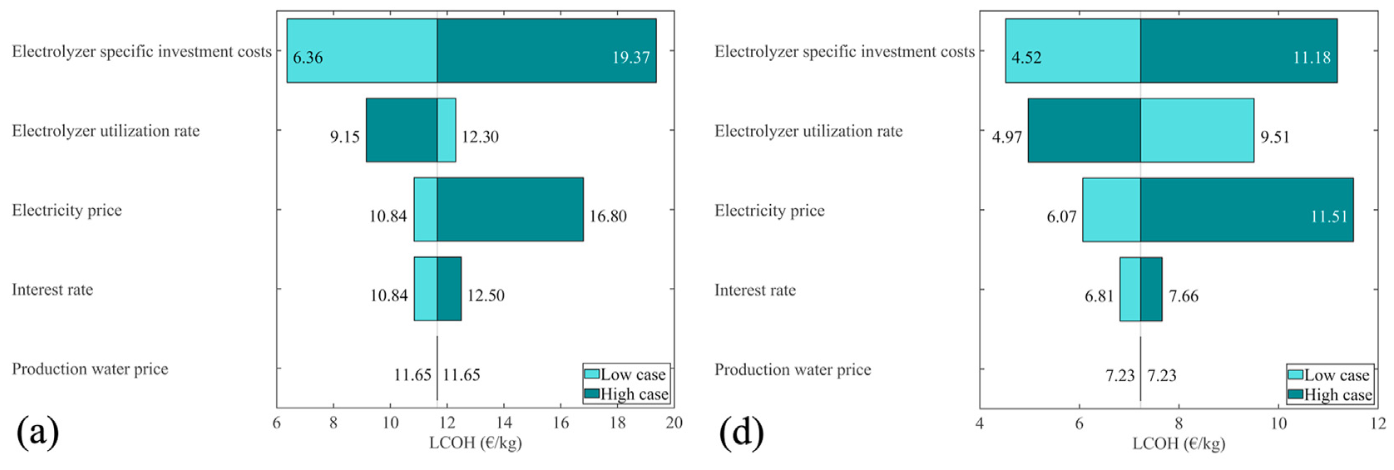
\includegraphics[width=\textwidth]{mmc-results-tornados-1.png}
		\end{center}
		\caption{Analiza wrażliwości -- scenariusz 1 (lewo - PV, prawo - wiatr)}
	\end{figure}
\end{frame}

\begin{frame}[noframenumbering]
	\frametitle{Analiza wrażliwości}
	\begin{figure}
		\begin{center}
			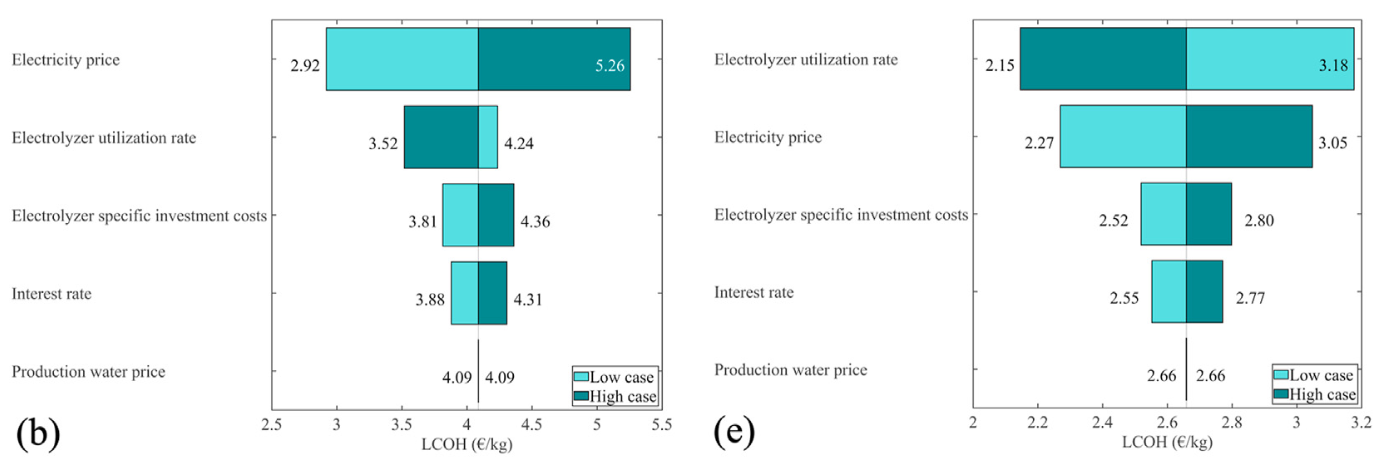
\includegraphics[width=\textwidth]{mmc-results-tornados-2.png}
		\end{center}
		\caption{Analiza wrażliwości -- scenariusz 2 (lewo - PV, prawo - wiatr)}
	\end{figure}
\end{frame}

\begin{frame}[noframenumbering]
	\frametitle{Analiza wrażliwości}
	\begin{figure}
		\begin{center}
			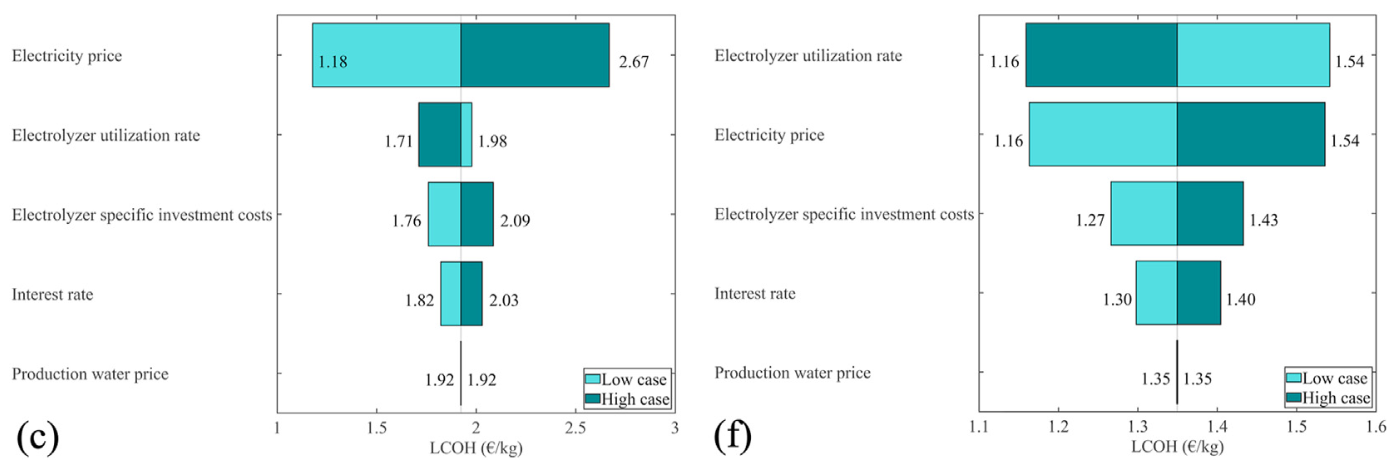
\includegraphics[width=\textwidth]{mmc-results-tornados-3.png}
		\end{center}
		\caption{Analiza wrażliwości -- scenariusz 3 (lewo - PV, prawo - wiatr)}
	\end{figure}
\end{frame}

\section{Podsumowanie}

\begin{frame}
	\frametitle{Dodatkowe uwagi}
	\begin{itemize}
		\con brak specyfikacji generatora liczb pseudolosowych
		\con miejscami nieprzyjemna kompozycja (w kilku rozdziałach to samo,
		przeplatane wykresy)
		\pro duża większość założeń ma źródła
		\pro wartości parametrów/zmiennych mają źródła
		\pro brak błędów ortograficznych, językowych, itp.
		\pro słowniczek skrótów na początku
		\pro dobrze sformatowane
	\end{itemize}
\end{frame}

\begin{frame}
	\frametitle{Subiektywna ocena}
	\begin{itemize}
		\item uzasadniona motywacja
		\item ładny język, dobrze sie czytało (nie licząc kompozycji)
		\item mógłby być krótszy
		\item \textbf{brak reprodukowalności}
	\end{itemize}
\end{frame}

\begin{frame}[allowframebreaks,noframenumbering]
	\frametitle{Bibliografia}
	\nocite{*} % Print all entries
	\printbibliography[heading=none]
\end{frame}


\begin{frame}[noframenumbering]
	\frametitle{Testy}
	\begin{itemize}
		\item Silnik testowany jednostkowo
		\item Moduł dekodujący i pliki zasad testowane integracyjnie, wraz z silnikiem
		\item Serwis API testowany integracyjnie wraz z pozostałymi komponentami
		\item Testy manualne
	\end{itemize}
\end{frame}


\end{document}
